\documentclass[a4paper,oneside,12pt]{book}
%% === nezbytné balíčky:
\usepackage[T1]{fontenc}    % kódování písma
%\usepackage[IL2]{fontenc}  % kódování písma
\usepackage{graphicx}
\usepackage[utf8]{inputenc}     % vstupní znaková sada tohoto dokumentu: UTF-8
%\usepackage[cp1250]{inputenc}  % vstupní znaková sada tohoto dokumentu: Windows 1250
%\usepackage[latin2]{inputenc}  % vstupní znaková sada tohoto dokumentu: ISO Latin 2
\usepackage{siunitx}
\usepackage[czech]{babel} % česky psaná práce, typografická pravidla. 
\usepackage{amsmath}
\usepackage{listings}
\usepackage{listings}
\usepackage{xcolor}

\definecolor{codegray}{rgb}{0.5,0.5,0.5}
\definecolor{codeblue}{rgb}{0,0,1}
\definecolor{codegreen}{rgb}{0,0.6,0}

\lstdefinelanguage{yaml}{
  morekeywords={true,false,null,yes,no,code,keywords,land_use, URL,buffer_layers,input_layer_name,controlling_atr_name,buffer_levels,priority,values,distance,default_buffer, layers, name,base_use_code,controlling_attribute,value_increments, N, J, L, S, layer_name},
  sensitive=false,
  morecomment=[l]{\#},
  morestring=[b]",
  morestring=[b]',
  alsoletter={:\-},       
  moredelim=[s][\color{codeblue}]{:}{\ },
  moredelim=[l][\color{codegray}]{\#}
}

\lstdefinestyle{myyaml}{
    language=yaml,
    basicstyle=\ttfamily\footnotesize,
    keywordstyle=\color{codeblue}\bfseries,
    commentstyle=\color{codegray},
    stringstyle=\color{codegreen},
    breaklines=true,
    numbers=left,
    numberstyle=\tiny\color{codegray},
    frame=single
}

\lstset{
  inputencoding=utf8,
  extendedchars=true,
  literate={á}{{\'a}}1 {č}{{\v{c}}}1 {ď}{{\v{d}}}1 {é}{{\'e}}1
           {ě}{{\v{e}}}1 {í}{{\'i}}1 {ň}{{\v{n}}}1 {ó}{{\'o}}1
           {ř}{{\v{r}}}1 {š}{{\v{s}}}1 {ť}{{\v{t}}}1 {ú}{{\'u}}1
           {ů}{{\r{u}}}1 {ý}{{\'y}}1 {ž}{{\v{z}}}1
           {Á}{{\'A}}1 {Č}{{\v{C}}}1 {Ď}{{\v{D}}}1 {É}{{\'E}}1
           {Ě}{{\v{E}}}1 {Í}{{\'I}}1 {Ň}{{\v{N}}}1 {Ó}{{\'O}}1
           {Ř}{{\v{R}}}1 {Š}{{\v{S}}}1 {Ť}{{\v{T}}}1 {Ú}{{\'U}}1
           {Ů}{{\r{U}}}1 {Ý}{{\'Y}}1 {Ž}{{\v{Z}}}1,
  style=myyaml
}

\lstdefinestyle{mypython}{
    language=Python,
    basicstyle=\ttfamily\footnotesize,
    keywordstyle=\color{codeblue}\bfseries,
    commentstyle=\color{codegray},
    stringstyle=\color{codegreen},
    breaklines=true,
    numbers=left,
    numberstyle=\tiny\color{codegray},
    frame=single
}
\lstset{
  inputencoding=utf8,
  extendedchars=true,
  literate={á}{{\'a}}1 {č}{{\v{c}}}1 {ď}{{\v{d}}}1 {é}{{\'e}}1
           {ě}{{\v{e}}}1 {í}{{\'i}}1 {ň}{{\v{n}}}1 {ó}{{\'o}}1
           {ř}{{\v{r}}}1 {š}{{\v{s}}}1 {ť}{{\v{t}}}1 {ú}{{\'u}}1
           {ů}{{\r{u}}}1 {ý}{{\'y}}1 {ž}{{\v{z}}}1
           {Á}{{\'A}}1 {Č}{{\v{C}}}1 {Ď}{{\v{D}}}1 {É}{{\'E}}1
           {Ě}{{\v{E}}}1 {Í}{{\'I}}1 {Ň}{{\v{N}}}1 {Ó}{{\'O}}1
           {Ř}{{\v{R}}}1 {Š}{{\v{S}}}1 {Ť}{{\v{T}}}1 {Ú}{{\'U}}1
           {Ů}{{\r{U}}}1 {Ý}{{\'Y}}1 {Ž}{{\v{Z}}}1,
  style=mypython
}


%Překládejte pomocí "latex.exe" nebo "pdflatex.exe"
%\usepackage{czech} % česky psaná práce. Překládejte pomocí "pdfCSlatex.exe" ("cslatex.exe" asi bude mít problém s balíkem geometry)
\usepackage{hhline} % Add the hhline package
\usepackage[a4paper, hmarginratio=3:2]{geometry} % využití A4 stránky a nastavení okrajů (u vazby bude širší)
\usepackage{afterpage}
\usepackage{caption}
\usepackage{pdfpages} % pokud nemáte formulář "Zadání bak./dipl. práce" naskenovaný jako PDF, tak ZAKOMENTUJTE
\usepackage[hidelinks]{hyperref} % v PDF budou klikací odkazy ("hidelinks" je nebude rámovat)
%% === balíčky, které se mohou hodit:
%\usepackage{encxvlna} % postará se o spojky a předložky, které dle českých pravidel nesmí být na konci řádku. Dokumentace: http://texdoc.net/texmf-dist/doc/generic/encxvlna/encxvlna.pdf (chová se správně k "vnitřku" listings?)

\usepackage{graphicx} % balíček pro vkládání rastrových grafických souborů (PNG apod.)
%\usepackage{epsfig} % balíčky pro vkládání grafických souborů typu EPS
\usepackage{float} % rozšířené možnosti umístění obrázků

%\usepackage{caption} % pro popisky obrázků, tabulek atd.

\usepackage{tabularx} % rozšířené možnosti tabulek
%\usepackage{tabu} % jiný balík pro rozšířené možnosti tabulek

\usepackage{listings}  % balíček vhodný pro ukázky zdrojového kódu v~textu práce/příloh. Nutno nastavit! http://ftp.cvut.cz/tex-archive/macros/latex/contrib/listings/listings.pdf
\usepackage{amsmath} % balíček pro pokročilou matematickou sazbu
%\usepackage{color} % pro možnost barevného textu
%\usepackage{fancybox} % umožňuje pokročilé rámečkování

%\usepackage{index} % nutno použít v případě tvorby rejstříku balíčkem makeindex
%\newindex{default}{idx}{ind}{Rejstřík} % zavádí rejstřík v případě použití balíku index

\renewcommand{\lstlistingname}{Kód}

\frenchspacing % za větou bude mezislovní mezera (v anglických textech je mezera za větou delší)
\widowpenalty=1000 % "síla" zákazu vdov (= jeden řádek ze začátku odstavce na konci stránky)
\clubpenalty=1000 % "síla" zákazu sirotků (= jeden řádek/slovo z konce odstavce samostatně na začátku stránky)
\brokenpenalty=1000 % "síla" zákazu zlomu stránky za řádkem, který má na konci rozdělené slovo

\topmargin=-15mm      % horní okraj trochu menší
\textwidth=150mm      % šířka textu na stránce
\textheight=240mm     % "výška" textu na stránce


\pagenumbering{arabic} % číslování stránek arabskými číslicemi
\pagestyle{plain}      % stránky číslované dole uprostřed

\parindent=0pt % odsazení 1. řádku odstavce
\parskip=7pt   % mezera mezi odstavci

\newcommand{\ti}{\textit} % zkrácený příkaz pro kurzívu
\newcommand{\tb}{\textbf} % zkrácený příkaz pro tučné písmo








%% --- zde jsou zavedeny některé "konstanty" - některé musíte změnit! --- %%
\newcommand{\cvut}{České vysoké učení technické v~Praze}
\newcommand{\fjfi}{Fakulta stavební}
\newcommand{\ksi}{Katedra geomatiky}
\newcommand{\program}{Geodézie a kartografie} % změňte, pokud máte jiný stud. program
\newcommand{\obor}{} % změňte, pokud máte jiný obor

\newcommand{\druh}{Diplomová práce} % nebo "Diplomová práce"
\newcommand{\woman}{} % pokud jste ŽENA, ZMĚŇTE na: ...{\woman}{a} (je to do Prohlášení)

\newcommand{\logoCVUT}{
\includegraphics{pictures/symbol_cvut_konturova_verze_cb.pdf}} % logo ČVUT -- podle grafického manuálu ČVUT platného od prosince 2016. Pokud nevyhovuje PDF-verze, tak použijte jinou variantu loga: https://www.cvut.cz/logo-a-graficky-manual -> "Symbol a logo ČVUT v Praze"). Pokud chcete logo úplně vynechat, zadejte místo "\includegraphics{...}" text "\vspace{35mm}"

% přesně podle formuláře "Zadání bak./dipl. práce" VYPLŇTE:
\newcommand{\nazevcz}{Vývoj zásuvného modulu QGIS pro určení využití území a potřeby analýz odtokových poměrů}    % český název práce (přesně podle zadání!)
\newcommand{\nazeven}{Development of a QGIS Plugin for Land Use Determination and Purposes of Runoff Analysis}          % anglický název práce (přesně podle zadání!)
\newcommand{\autor}{Bc. Josef Jehlička}   % vyplňte své jméno a příjmení (s akademickým titulem, máte-li jej)
\newcommand{\vedouci}{Ing. Martin Landa, Ph.D. } % vyplňte jméno a příjmení vedoucího práce, včetně titulů, např.: Doc. Ing. Ivo Malý, Ph.D.
\newcommand{\druhyvedouci}{doc. Ing. Petr Kavka, Ph.D.}
\newcommand{\pracovisteVed}{\ksi, \fjfi, \cvut} % ZMĚŇTE, pokud vedoucí Vaší práce není z KSI
\newcommand{\konzultant}{--} % POKUD MÁTE určeného konzultanta, NAPIŠTE jeho jméno a příjmení
\newcommand{\pracovisteKonz}{--} % POKUD MÁTE konzultanta, NAPIŠTE jeho pracoviště

% podle skutečnosti VYPLŇTE:
\newcommand{\rok}{2025}  % rok odevzdání práce (jen rok odevzdání, nikoli celý akademický rok!)
\newcommand{\kde}{Praze} % studenti z Děčína ZMĚNÍ na: "Děčíně" (doplní se k "prohlášení")

\newcommand{\klicova}{Klíčová slova}   % zde NAPIŠTE česky max. 5 klíčových slov
\newcommand{\keyword}{Key words}       % zde NAPIŠTE anglicky max. 5 klíčových slov (přeložte z češtiny)
\newcommand{\abstrCZ}{Popis práce česky}    % zde NAPIŠTE abstrakt v češtině (cca 7 vět, min. 80 slov)
\newcommand{\abstrEN}{Popis práce anglicky} % zde NAPIŠTE abstrakt v angličtině

\newcommand{\prohlaseni}{Prohlašuji, že jsem diplomovou práci s názvem "Vývoj QGIS zásuvného modulu pro potřeby výpočtu objemu přímého odtoku metodou SCS-CN“ vypracoval samostatně s odborným vedením pana Ing. Martina Landy, Ph.D a doc. Ing. Petra Kavky, Ph.D. Použitá literatura a další podklady, které byly použity pro tuto diplomovou práci, jsou uvedeny v seznamu literatury. 
} % text prohlášení můžete mírně upravit :-)

\newcommand{\podekovani}{Tímto bych chtěl poděkovat } % NAPIŠTE poděkování, např. svému vedoucímu:
% Děkuji Ing. Eleonoře Krtečkové, Ph.D. za vedení mé bakalářské práce a za podnětné návrhy, které ji obohatily.
% NEBO:
% Děkuji vedoucímu práce doc. Pafnutijovi Snědldítětikaši, Ph.D. za neocenitelné rady a pomoc při tvorbě bakalářské práce.













\begin{document}
%%%%%%%%%%%% TITULNÍ STRANA -- na následujících cca 30 řádků NESAHEJTE!!!  Generuje se AUTOMATICKY %%%%%%%%%%%%
\thispagestyle{empty}

\begin{center}
	{\LARGE
		\cvut\par
		\fjfi
	}
    \vspace{10mm}

    \begin{tabular}{c}
		\tb{\ksi} \\[3pt]   
		\tb{Program: \program}\\
    \end{tabular}

   \vspace{10mm} \logoCVUT \vspace{15mm} 

   {\huge \tb{\nazevcz}\par}
   \vspace{5mm}   
   {\huge \tb{\nazeven}\par}
   
   \vspace{15mm}
   {\Large \MakeUppercase{\druh}}

   \vfill
   {\large
    \begin{tabular}{ll}
    Vypracoval: & \autor\\
    Vedoucí práce: & \vedouci\\
    & \druhyvedouci \\
    Rok: & \rok
    \end{tabular}
   }
\end{center}



%%%%%%%%%%%% ZADÁNÍ PRÁCE %%%%%%%%%%%%
% Zadání (podepsané děkanem!) musíte NASKENOVAT. Ideálně jako 2stránkové PDF (soubor "zadani_cele.pdf"). 
% Před svázáním to v jednom výtisku VYMĚNÍTE ZA ORIGINÁLNÍ ZADÁNÍ (podepsané děkanem fakulty)!
\newpage  % SEM NESAHEJTE!
\thispagestyle{empty} % SEM NESAHEJTE!

%% zde podle toho, jak jste zadání naskenovali, VYBERTE variantu A, B nebo C:
%
% --- varianta A: zadání naskenované jako 2stránkové PDF:




 % 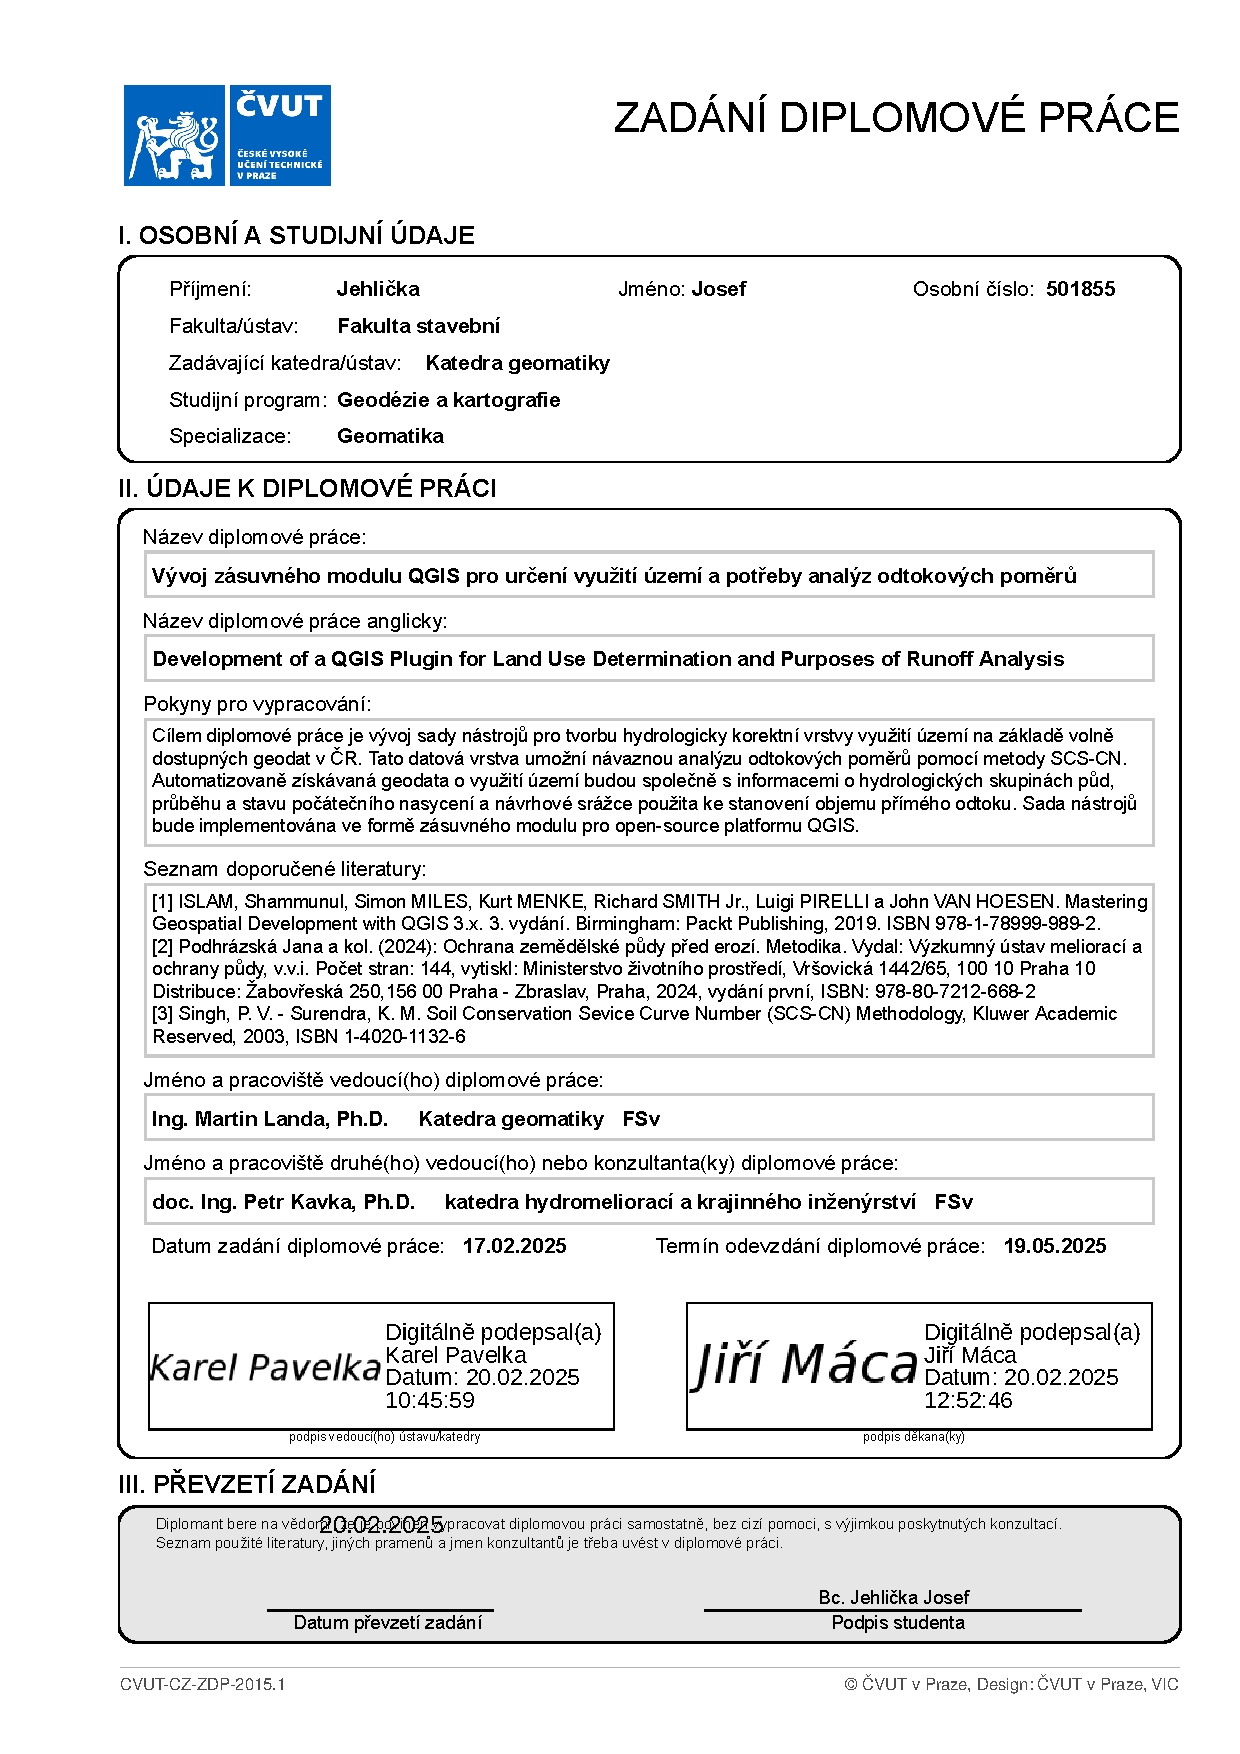
\includepdf[pages={1}]{zadani_cele.pdf} % NAHRAĎTE správným souborem! <<<<<<<<<<<<<<<<<<<<<<<<<





%
%% --- varianta B: zadání naskenované jako jednotlivé stránky:
%\includepdf[pages={1}]{zadani1.pdf} % 1. strana zadání v PDF
%\includepdf[pages={1}]{zadani2.pdf} % 2. strana zadání v PDF
%
%% --- varianta C: zadání naskenované jako 2 samostatné obrázky:
%% 1. strana zadání
%\begin{center}
%     \includegraphics[width=1\textwidth]{zadani1.jpg}
%\end{center}
%% 2. strana zadání
%\newpage  % SEM NESAHEJTE!
%\thispagestyle{empty} % SEM NESAHEJTE!
%\begin{center}
%     \includegraphics[width=1\textwidth]{zadani2.jpg}
%\end{center}







% příprava:    (na následujících 8 řádků NESAHEJTE!)
\newbox\odstavecbox
\newlength\vyskaodstavce
\newcommand\odstavec[2]{%
    \setbox\odstavecbox=\hbox{%
         \parbox[t]{#1}{#2\vrule width 0pt depth 4pt}}%
    \global\vyskaodstavce=\dp\odstavecbox
    \box\odstavecbox}
\newcommand{\delka}{120mm} % šířka textů ve 2. sloupci tabulky

% použití přípravy:    % dovnitř "tabular" vůbec NESAHEJTE!

\section*{ABSTRAKT}
\begin{flushleft}
Tato práce popisuje vývoj zásuvného modulu open-source softwaru QGIS, který provádí přípravu dat a následnou analýzu odtoků SCS-CN  na automatizovaně získávaných volně dostupných geo datech v ČR jako jsou ZABAGED, LPIS a data poskytovaná projektem rain.fsv.cvut.cz. Data jsou ohodnocena podle způsobu využití území a v kombinaci s daty hydrologických skupin půd a hodnotou úhrnu návrhové srážky vstupují do následné analýzy.
\end{flushleft}


\section*{KLÍČOVÁ SLOVA}
\begin{flushleft}
QGIS, SCS-CN, využití území, zásuvný modul, Python, odtok, povodí, GIS, ZABAGED, LPIS
\end{flushleft}


\section*{ABSTRACT}
\begin{flushleft}
This master's thesis describes the development of a plugin for the open-source software QGIS, which performs data preparation and subsequent runoff analysis using the SCS-CN method on automatically acquired freely available geodata in the Czech Republic, such as ZABAGED, LPIS  and data provided by the rain.fsv.cvut.cz project. The data are evaluated based on land use and, in combination with data of hydrologic soil groups and the total design rainfall amount, serve as inputs for the subsequent analysis.
\end{flushleft}


\section*{KEY WORDS}
\begin{flushleft}
QGIS, SCS-CN, land use, plugin, Python, runoff, watershed, GIS, ZABAGED, LPIS
\end{flushleft}

















%%%%%%%%%%%% Prohlášení -- SEM NESAHEJTE! Generuje se automaticky z výše nastavených maker \kde{} a \prohlaseni{}. %%%%%%%%%%%%
\newpage % SEM NESAHEJTE!
\thispagestyle{empty}  % SEM NESAHEJTE!

~ % SEM NESAHEJTE!
\vfill % prázdné místo. SEM NESAHEJTE!
\vspace{1em}
\tb{Prohlášení} % SEM NESAHEJTE!

\vspace{1em} % vertikální mezera. SEM NESAHEJTE!
\prohlaseni

\vspace{2em}  % SEM NESAHEJTE!
\hspace{-0.5em}\begin{tabularx}{\textwidth}{X c}  % SEM NESAHEJTE!
V \kde\ dne .................... &........................................ \\	% SEM NESAHEJTE!
	& \autor
\end{tabularx}	% SEM NESAHEJTE!







\newpage % SEM NESAHEJTE!
\thispagestyle{empty}  % SEM NESAHEJTE!

~
\vfill % prázdné místo


% -- následující kus kódu (do "%%%%%%%%%%%% ABSTRAKT") můžete odstranit, pokud nechcete psát poděkování:
\vspace{1em}
\tb{Poděkování}

\vspace{1em} % vertikální mezera
\podekovani
\begin{flushright}
\autor
\end{flushright}  % <------- tady končí stránka s poděkováním





\newpage
\chapter*{Obsah}




\newpage
\chapter*{Úvod} \label{uvod}
Technologie GIS usnadňuje práci v nejrůznějších odvětví průmyslu od precizního zemědělství až po působení bezpečnostních složek. Což může být motivací pro ušlechtilé úsilí určité skupiny vývojářů, takovou pomoc poskytnout zdarma jako otevřený software s možností dodatečného přizpůsobení nebo integrace do externích aplikací. 

Tvorbou zásuvného modulu (pluginu) pro GIS s otevřeným zdrojovým kódem QGIS se zabývá i tato práce. Zmíněný zásuvný modul poskytuje možnost usnadnit práci uživatelům působícím v oblasti hydrologie, konkrétně při výpočtu objemu přímého odtoku metodou SCS-CN na území České Republiky. Takové modelování může například být využito při vymezování záplavových území nebo návrzích protipovodňových opatření.

Cílem bylo vytvořit nástroj pro získání dat, ohodnocení území dle jeho využití, kombinaci těchto dat s vrstvou hydrologických skupin půd, doplnění hodnot CN z tabulky a z nich získání objemu přímého odtoku. Uživateli je umožněno v každé části procesu editovat jakékoliv vstupní hodnoty, či upravit nebo použít vlastní geo data. Tento zásuvný modul realizovaný pomocí programovacího jazyka Python je doplněn o dokumentaci a softwarové testy. 

Ačkoliv existují komerční nástroje pro modelování odtokových poměrů metodou SCS-CN, v prostředí volně dostupných GIS řešení chybí specializovaný nástroj, který by kombinoval snadnou použitelnost, integraci s českými datovými zdroji a možnost úprav vstupních parametrů.

Samotná práce popisuje metodu odtokových křivek SCS-CN, software QGIS a s ním propojené softwarové nástroje jako jsou WFS, WPS, jazyk YAML, knihovna PyQt a další. Následně se pak zaměřuje na  datové zdroje volně dostupně v České Republice, kterými jsou ZABAGED a LPIS. Obsahuje též popis prací při vývoji zásuvného modulu. Závěrečná část shrnuje dosažené výsledky, zhodnocuje přínos práce a nabízí možnosti dalšího rozšíření.



\newpage
\chapter{Meotda SCS-CN} \label{SCSCN}
\hspace{10mm} Metoda odtokových křivek (SCS-CN) se používá pro určení objemu přímého odtoku při návrhových přívalových deštích. Výhody této metody spočívají v její jednoduchosti a schopnosti reagovat na vlastnosti povodí jako je typ půdy či využití pozemku (land use). Metoda byla vyvinuta v roce 1954 a publikována v roce 1986 organizací USDA Natural Resources Conservation Service (dříve nazývána Soil Conservation Service). [1] Vývoj probíhal na empirických datech získaných v USA, nicméně později byla modifikována na různé typy využití pozemku typické i pro jiné podmínky. [2][3]

\hspace{10mm} Tato metoda může být využita i v menších částech jednotlivých povodí, jejichž rozloha by neměla překročit 10 $km^{2}$ a není vhodná pro výpočet odtoku z tání sněhu. V České republice se využívá hlavně pro návrhy protierozních opatření, a to v souladu s ČSN 75 1300. [4]

Výstupem metody CN křivek je hodnota efektivní srážkové výšky dle vzorce (1) [5]:


\begin{equation}
H_{0} = \frac{\displaystyle (H_{S} - I_{a})^{2}}{\displaystyle H_{S} - I_{a} + A}
\end{equation}

kde:
\begin{tabbing}
    \hspace{10mm} \= $H_{0}$ \hspace{5mm} \= je výška přímého odtoku (mm) \\
    \> $H_{s}$ \> je celkový srážkový úhrn (mm) \\
    \> $I_{a}$ \> je počáteční ztráta (mm) \\
    \> $A$ \> je maximální potenciální retence (mm)
\end{tabbing}

Hodnota počáteční ztráty ($I_{a}$) se určí jako:
\begin{equation}
I_{a} = \lambda A
\end{equation}

\hspace{10mm} Kde $\lambda$ je poměrový koeficient, který se v základu volí $0.2$. Tato hodnota byla empiricky odvozena na povodích na území USA. [3][5] Takto zvolená hodnota se stala jedním důvodem pro kritiku této metody. [1] \\

\hspace{10mm} Maximální potenciální retence ($A$) je dále určena na základě CN (curvature number) křivek ze vztahu [4] : 
\begin{equation}
A = 25,4 (\frac{1000}{CN}-10)
\end{equation}
\hspace{10mm} Hodnota CN se pohybuje mezi 0 (prakticky 30) až 100. Čím vyšší je hodnota CN, tím větší je pravděpodobnost, že dojde k povrchovému odtoku. Pokud se CN rovná nule, potom představuje teoretickou horní
hranici potenciální retence, což by znamenalo, že takové povodí je nekonečně propustné. [6]

\begin{figure}[ht] \label{obr1}
\centering
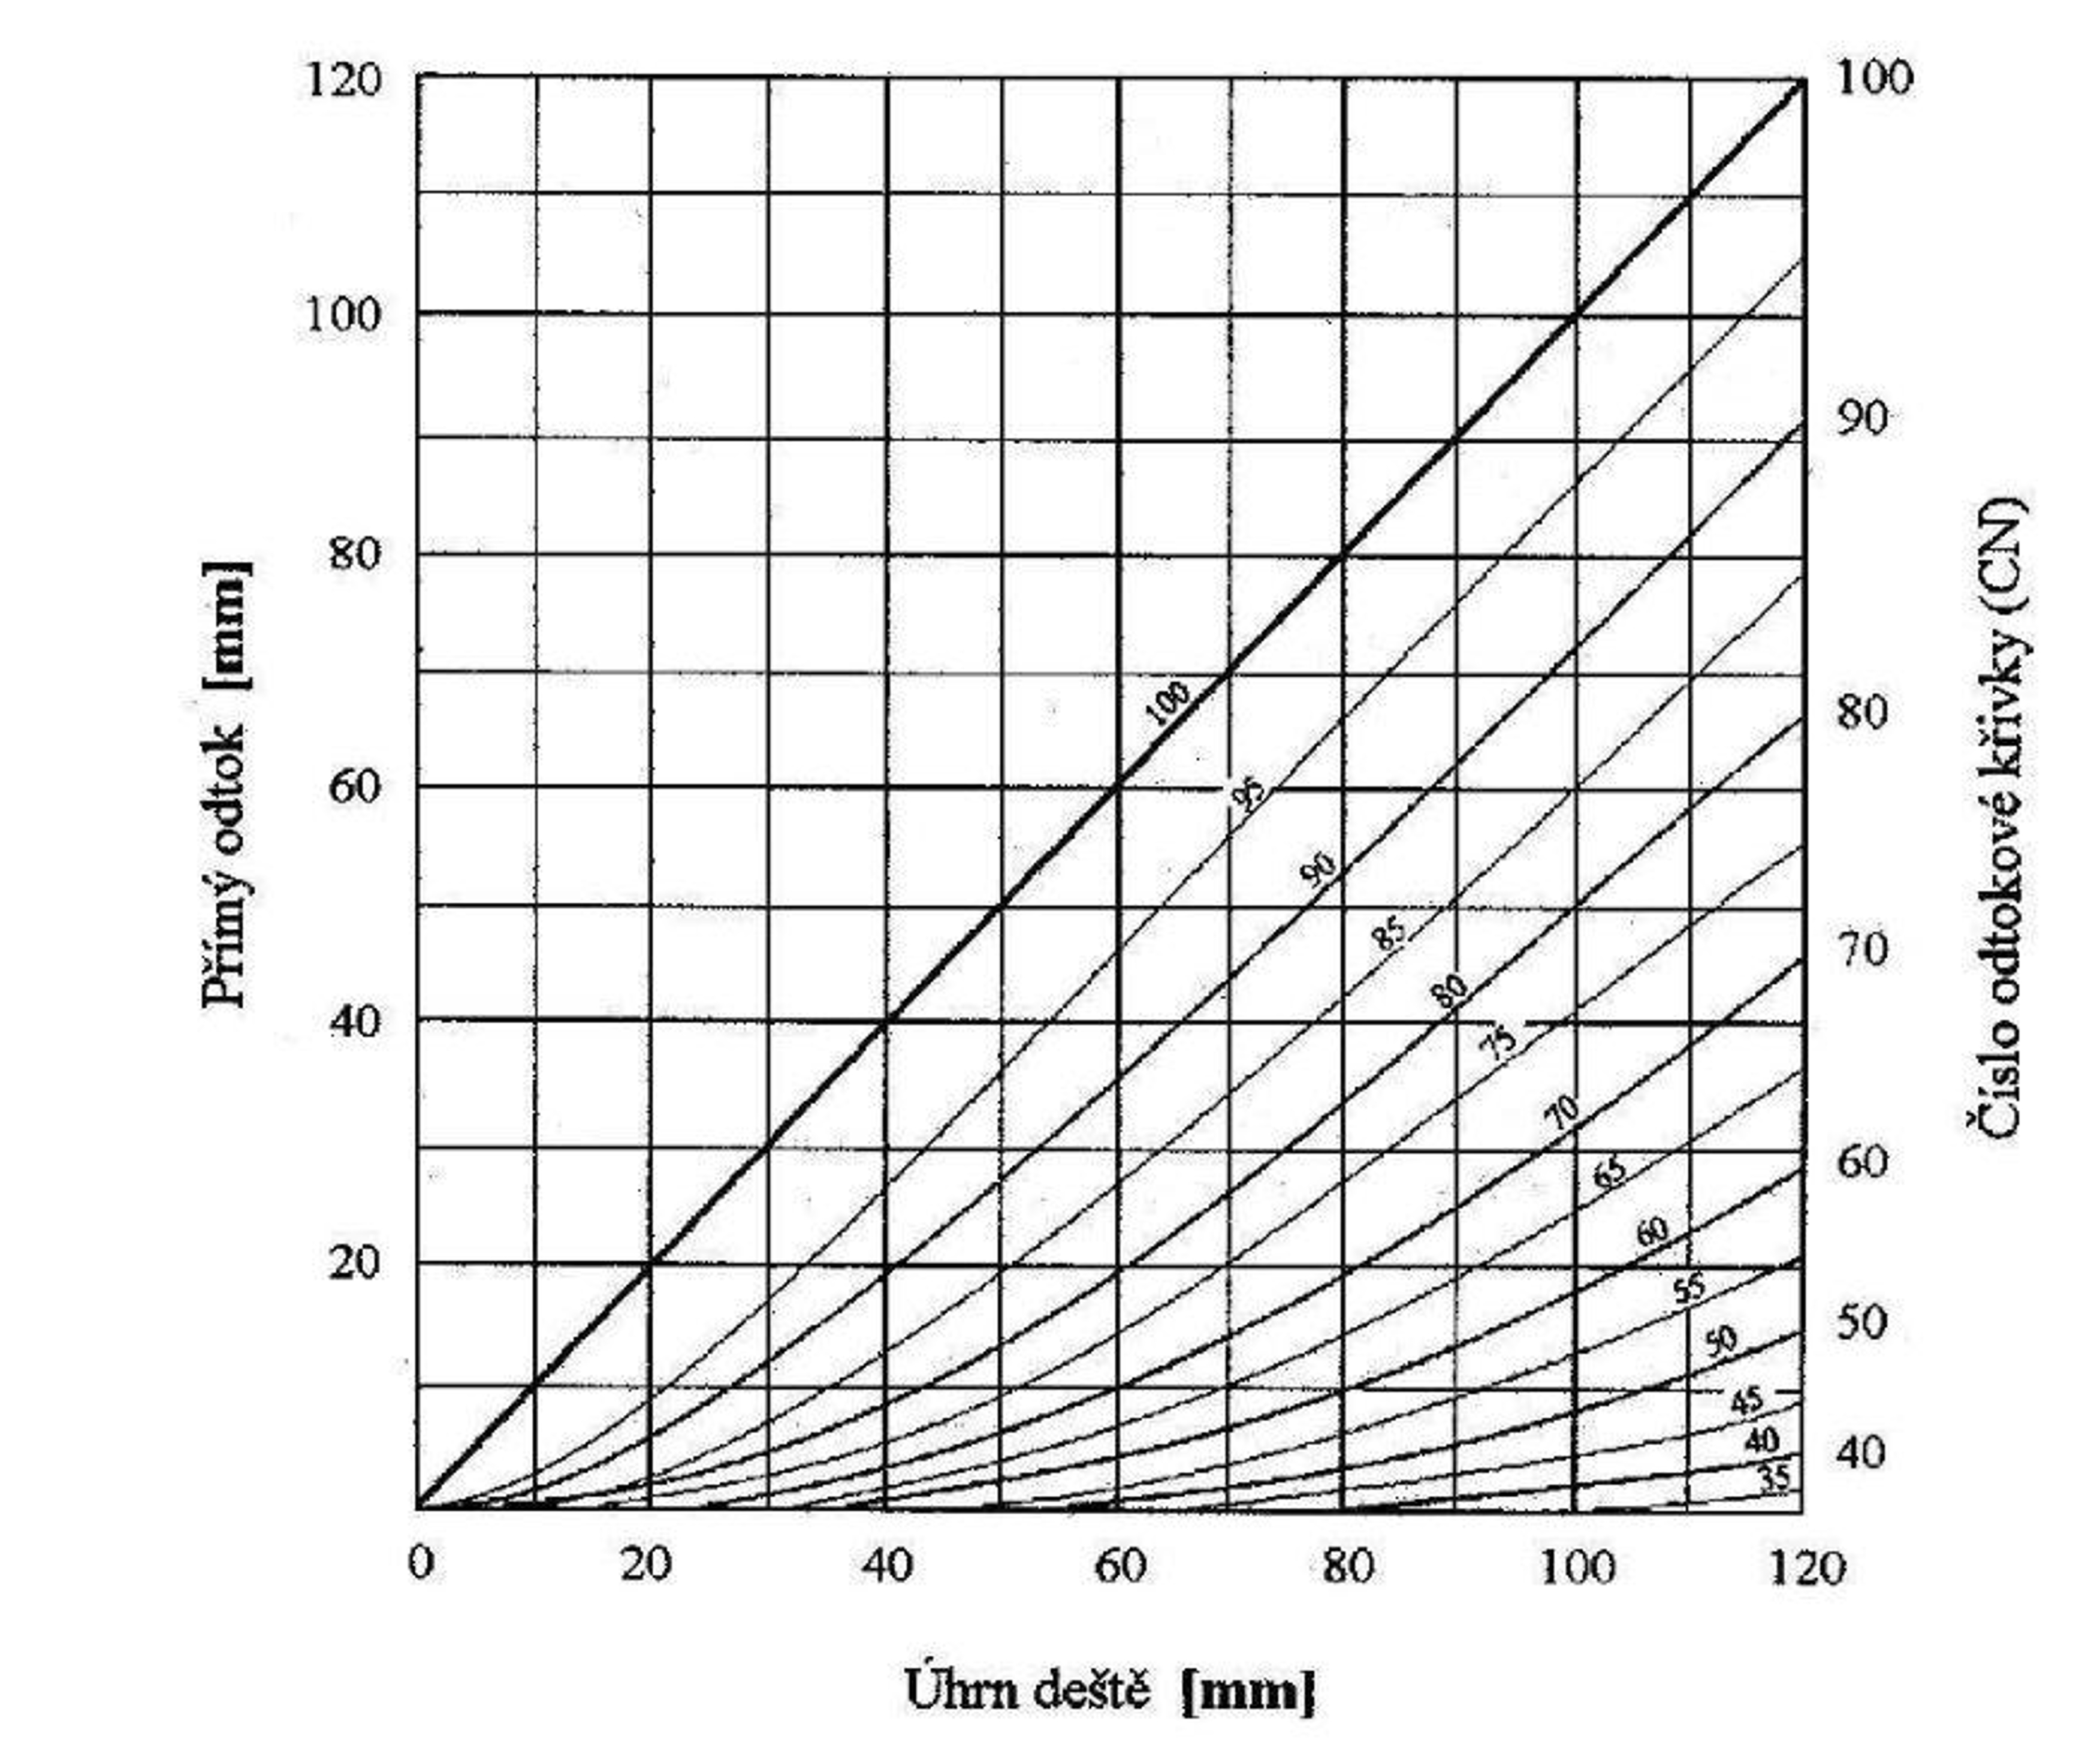
\includegraphics[height=12cm]{pictures/CNcurves.jpg}
\caption{ Závislost výšky přímého odtoku ($H_{o}$) na úhrnu deště($H_{S}$) a číslech odtokových křivek (CN) [4]}
\label{fig:example}
\end{figure}

 \hspace{10mm} Tato čísla jsou tabelována pro dvojici jevů. Těmi jsou hydrologické skupiny půd (HSP) a způsob využití území (land use) případně doplněn o počáteční vlhkostní podmínky. [6][7]

\hspace{10mm} Hydrologické skupiny půd (HSP) existují čtyři: A,B,C,D. Do těchto skupin se řadí půda dle minimálních rychlostí infiltrace vody do půdy bez pokryvu a po dlouhodobém nasycení.[4]
\begin{table}[htbp]
  \centering
  \caption{Tabulka rozdělení do hydrologických skupin půd (HSP) [4]} 
  \label{tab:HSP}
  \begin{tabular}{|c|p{6cm}|p{2.5cm}|p{2.5cm}|}
    \hline
    Skupina & Charakteristika hydrologických vlastností [m] & 
    Rychlost infiltrace [mm.min\textsuperscript{-1}] & Rychlost infiltrace [mm.den\textsuperscript{-1}] \\
    \hhline{=|=|=|=|}
    A & Půdy s vysokou rychlostí infiltrace i při úplném nasycení, zahrnující převážně hluboké, dobře až nadměrně odvodněné písky nebo štěrky. & > 0,12 & > 172 \\
    \hline
    B & Půdy se střední rychlostí infiltrace i při úplném nasycení, zahrnující převážně půdy středně hluboké až hluboké, středně až dobře odvodněné, hlinitopísčité až jílovitohlinité. & 0,06–0,12 & 86,4–172 \\
    \hline
    C & Půdy s nízkou rychlostí infiltrace i při úplném nasycení, zahrnující převážně půdy s málo propustnou vrstvou v půdním profilu a půdy jílovitohlinité až jílovité. & 0,02–0,06 & 28,8–86,4 \\
    \hline
    D & Půdy s velmi nízkou rychlostí infiltrace i při úplném nasycení, zahrnující především jíly s vysokou bobtnavostí, půdy s trvale vysokou hladinou podzemní vody, půdy s vrstvou jílu na povrchu nebo těsně pod ním a mělké půdy nad téměř nepropustným podložím. & < 0,02 & < 28,8 \\
    \hline
  \end{tabular}
  
\end{table}

% Různé zdroje půd (HSP) - velký rozdíl výsledků, je tam graf https://www.vodnihospodarstvi.cz/ArchivPDF/vh2022/vh_09-2022.pdf
\newpage
\chapter{QGIS} \label{qgis}
\hspace{10mm} QGIS (dříve známý jako Quantum GIS) je jeden z geografických informačních systémů (GIS), tj.  informační systém zabývající se informacemi, které se týkají jevů přidružených k místu vztaženému k Zemi.[8]

\begin{figure}[ht] \label{obr2}
\centering

\includegraphics[height=2cm]{pictures/qgis-logo.png}
\caption{Logo softwaru QGIS}
\label{fig:QGIS}
\end{figure}

\hspace{10mm} Tento software je podporován v prostředí Windows,Mac OS, Linux i Unix. Na rozdíl od komerčních alternativ, jako je například ArcGIS, je QGIS zcela zdarma k použití a řadí se mezi takzvaný otevřený software, který je spravován neziskovou organizací The Open Source Geospatial Foundation (OSGeo).

\begin{figure}[ht] \label{obr3}
\centering

\includegraphics[height=2cm]{pictures/Osgeo.png}
\caption{ Logo organizace OSGeo}
\label{fig:OSGEO}
\end{figure}

\hspace{10mm} OSGeo stojí i za řadou dalších projektů na poli otevřeného softwaru, jako jsou například:
\begin{itemize}
\item GRASS GIS 
\item gvSIG - GIS software
\item PROJ - knihovna pro tansformaci souřadnic a kartografických projekcí
\item GDAL/OGR - knihovna pro čtení a zápis GIS formátů
\item PostGIS - SQL pro práci s geoprostorovými daty
\item GeoServer - Serverová platforma umožňující publikaci prostorových dat 
\item OpenLayers - JavaScript knihovna pro tvorbu webových mapových aplikací
\end{itemize}


\hspace{10mm} QGIS funguje pod licencí GNU GPL a je postaven na knihovně Qt jazyka C++. QGIS vznikal iniciativou Garyho Shermana, který ji započal v roce 2002 jako prohlížecí software geoprostorových dat pro operační systém Linux. Jeho první verze vyšla až v roce 2009. [9]

 \section{Zásuvné moduly} \label{moduly}

\hspace{10mm} QGIS je pravidelně jeho vývojáři rozšiřován o nejrůznější funkce, často přejímané z dalších otevřených softwarů jako je například: GRASS GIS, GDAL nebo SAGA GIS.[10]

\hspace{10mm} Nespornou výhodou je i fakt, že jakákoliv nezávislá organizace, či jednotlivec může vyvinout vlastní rozšíření tohoto softwaru pomocí zásuvných modulů (tzv. pluginů) využívajících QGIS Python API (PyQGIS). Pokud takto vytvořený modul splní požadavky OSGeo, může být vydán pod její záštitou. Jinak může být distribuován neoficiálně například v komprimovaném adresáři.

\hspace{10mm} Vytvoření takového pluginu zjednodušuje plugin již existující, a to Plugin Builder. Ten je vyvinut společností GeoApt LLC jejímž vlastníkem je již zmíněný Garry Sherman zakladatel samotného softwaru QGIS. Tento nástroj vytvoří šablonu potřebných souborů pro potřebu vytvoření zásuvného modulu. [11]

\hspace{10mm} Mezi další významné pluginy patří například: OpenLayers Plugin pro zobrazení vrstev Google Maps nebo OpenStreetMap, QuickMapServices pro načítání různých mapových služeb a datových setů, Semi-Automatic Classification Plugin pro řízenou klasifikaci družicových snímků nebo qgis2web pro exportování vrstev do formátu webových stránek. [11]



\chapter{Datové zdroje} \label{data}
\hspace{10mm} Vstupem pro metodu SCS-CN je kombinace informací o využití území a hydrologických skupinách půd v daném území. Vrstva využití území je v zásuvném modulu získána kombinací vrstev ZABAGED a LPIS. 

\section{ZABAGED\texorpdfstring{\textsuperscript{\textregistered}}{ (R)}} \label{zabaged}

\hspace{10mm} Základní báze geografických dat České republiky (ZABAGED\texorpdfstring{\textsuperscript{\textregistered}}{ (R)}) je vektorová geografická datová sada ve správě Zeměměřického úřadu ve veřejném zájmu. Skládá se z 140 různých polohopisných geografických objektů, které spadají do následujících kategorií [12] :
\begin{itemize}
\item 1. Sídla, hospodářské a kulturní objekty
\item 2. Komunikace
\item 3. Rozvodné sítě a produktovody
\item 4. Vodstvo 
\item 5. Územní jednotky včetně chráněných území
\item 6. Vegetace a povrch
\item 7. Terénní reliéf
\item 8. Geodetické body
\end{itemize}
\hspace{10mm} Kromě polohopisných dat obsahuje ZABAGED\texorpdfstring{\textsuperscript{\textregistered}}{ (R)} i data výškopisná (vrstevnice, DMR 4G, DMR 5G, DMP 1G) a data spadající pod rámec INSPIRE (Vodstvo, Dopravní sítě, Nadmořská výška GRID, Nadmořská výška TIN). [12] 


\hspace{10mm} Polohopisné objekty jsou distribuována v různých geometrických zobrazeních:
\begin{itemize}
\item bod
\item centroid plochy
\item linie
\item linie - osa objektu
\item obvodová linie
\item plocha
\end{itemize}

\hspace{10mm} Každý objekt obsahuje atribut o jeho střední polohové chybě vyjádřené v metrech. Původním zdrojem těchto polohových dat je Základní mapa České republiky 1:10 000 (ZM 10). Ta byla několikrát aktualizována pomocí aktuálního Ortofota ČR. Dále se v menší míře využívají data z přímého geodetického měření, data z leteckého laserového
skenování či data od externích subjektů. [12] 


\section{LPIS} \label{lpis}
\hspace{10mm} LPIS (Land Parcel Identification System) je geografický informační systém sloužící hlavně k evidenci zemědělské půdy, za který je odpovědné Ministerstvo zemědělství. Obsahem jsou zemědělské parcely zobrazující vlastnické vztahy. Ty jsou výchozí pro udělování dotací pro zemědělskou půdu.[13] 

\hspace{10mm} Základní datovou jednotkou je díl půdního bloku (DPB), které jsou zcelovány do souvislých obhospodařovaných ploch tzv. půdních bloků (PB).[13]

\hspace{10mm} LPIS je veden ve všech státech Evropské unie, ale v různých státech se pozemky uchovávají v jiných druzích parcel (katastrální parcely, zemědělské parcely, zemědělské půdní bloky nebo fyzické bloky). [14]

Takové plochy obsahují údaje o druhu zemědělské kultury, a to [15]:
\begin{itemize}
    \item orná půda, kterou je
    \begin{itemize}
        \item standardní orná půda,
        \item travní porost a
        \item úhor,
    \end{itemize}
    \item trvalý travní porost,
    \item trvalá kultura, kterou je
    \begin{itemize}
        \item vinice,
        \item chmelnice,
        \item ovocný sad,
        \item školka,
        \item rychle rostoucí dřeviny pěstované ve výmladkových plantážích,
        \item plocha s víceletými produkčními plodinami,
        \item plocha s lanýži a
        \item jiná trvalá kultura, 
    \end{itemize}
    \item ostatní kultura, kterou je
    \begin{itemize}
        \item zalesněná půda,
        \item rybník,
        \item plocha s kontejnery,
        \item mimoprodukční plocha a
        \item jiná kultura.
    \end{itemize}
\end{itemize}

\hspace{10mm} Databáze také obsahuje ekologicky významné prvky a další objekty. [15]
Přístup k těmto datům je zprostředkován webovými službami (iLPIS a pLPIS)  a WMS či WFS službou. [14]

\section{Hydrologické skupiny půd (HSP)} \label{hsp}
\hspace{10mm}Význam hydrologických skupin půd (hydrology soil groups) a jejich dělení je popsáno v první kapitole. 
% Různé zdroje půd (HSP) - velký rozdíl výsledků, je tam graf https://www.vodnihospodarstvi.cz/ArchivPDF/vh2022/vh_09-2022.pdf

Zdroje hydrologických skupin půd v České republice existují celkem čtyři[16]:
\begin{itemize}
\item CN (s metodikou výpočtu) dle ČHMÚ (2004)
\item HSP dle projektu „Strategie ochrany před negativními dopady povodní a erozními jevy přírodě blízkými opatřeními v České republice“ (2015)
\item HSP dle VÚMOP (2018) 
\item HSP dle půdní zrnitosti, dle projektu "Fyzikální a hydropedologické vlastnosti půd ČR" (2021)
\end{itemize}
\hspace{10mm} Volba zdroje půdních dat může ovlivnit výsledky analýz, nicméně neexistuje způsob, jak určit spolehlivost těchto rozdílných zdrojů dat, i přestože se poměrně značně liší.[16] To je vizualizováno níže.

\begin{figure}[ht] \label{obr4}
\centering
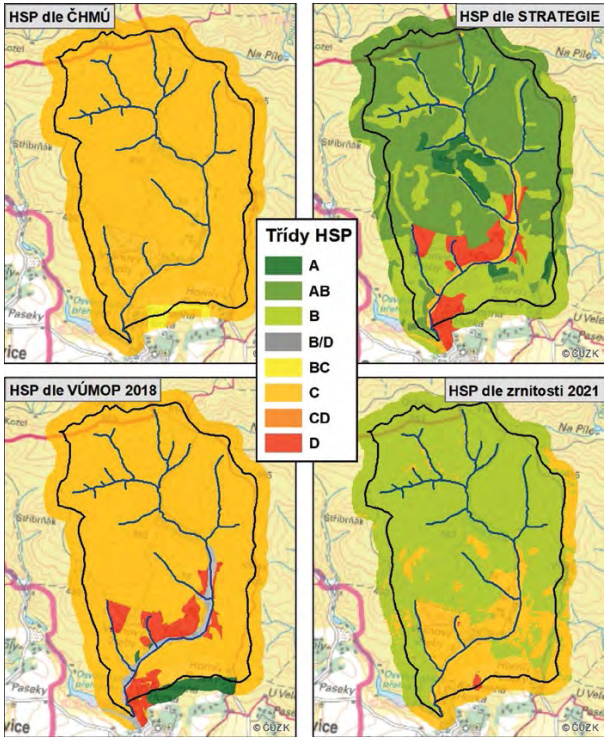
\includegraphics[height=12cm]{pictures/HSPmapa.png}
\caption{Plošné rozdělení jednotlivých HSP na povodí Hruškovice podle různých podkladů [16]}
\label{fig:hsp}
\end{figure}

\newpage
\newpage

\chapter{Použité technologie} \label{tehcnologie}

\section{Web Feature Service (WFS)} \label{wfs}
\hspace{10mm} Web Feature Service je internetová služba pro šíření geografických informací, která nahradila šíření celých datových souborů například pomocí File Transporn Protocol (FTP). Služba je standardizována organizací Open Geospatial Consortium (OGC) v dokumentu  ISO 19119. [17] WFS je napsáno v jazyce XML a data jsou reprezentována primárně v jazyce GML. [18]

\hspace{10mm} Na rozdíl od Web Map Service (WMS), která připojuje vrstvy jako needitovatelné rastrové podkladové vrstvy, WFS slouží ke sdílení vektorových dat s možností následné editace. Uživatel zašle požadavek ve formátu XML na WFS server, který vrátí odpověď opět V XML. [18]

\begin{figure}[ht] \label{obr5}
\centering
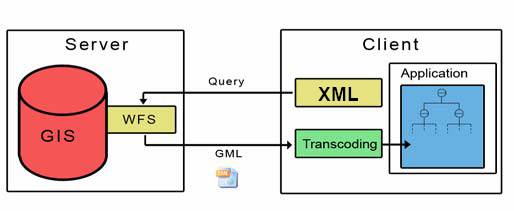
\includegraphics[height=6cm]{pictures/XML.png}
\caption{Schéma služby WFS [19]}
\label{fig:xml}
\end{figure}

\hspace{10mm} Pro komunikaci se serverem poskytující WFS službu může uživatel využít následujících jedenáct operací:

\begin{table}[htbp]
  \centering
  \caption{Tabulka WFS operací} 
  \label{tab:WFS}
  \begin{tabular}{|c|c|p{7cm}|}
    \hline
    \textbf{Operace} & \textbf{Volitelný} & \textbf{Popis} \\
    \hhline{=|=|=}
    GetCapabilities & NE & Načte metadata o službě, včetně podporovaných operací a parametrů, a seznam dostupných typů prvků. \\
    \hline
    DescribeFeatureType & NE & Vrací popis struktury typů prvků a jejich vlastností, které WFS poskytuje nebo přijímá. \\
    \hline
    GetFeature & NE & Vrací výběr instancí prvků z datového úložiště publikovaného prostřednictvím WFS. \\
    \hline
    ListStoredQueries & NE & Vrací seznam dotazů, které byly uloženy v instanci WFS. \\
    \hline
    DescribeStoredQueries & NE & Vrací popis dotazů, které byly uloženy v instanci WFS. \\
    \hline
    GetPropertyValue & ANO & Načítá hodnotu vlastnosti prvku nebo část hodnoty složité vlastnosti pro sadu prvků. \\
    \hline
    GetFeatureWithLock & ANO & Podobné jako GetFeature, ale s možností uzamknout prvek pro následné úpravy. \\
    \hline
    LockFeature & ANO & Uzamkne sadu instancí prvků tak, aby je jiné operace nemohly měnit, dokud je zámek aktivní. \\
    \hline
    Transaction & ANO & Umožňuje modifikaci nebo odstranění instancí prvků a jejich vlastností. \\
    \hline
    CreateStoredQuery & ANO & Vytvoří a uloží dotaz, který může klient snadno vyvolat později. \\
    \hline
    DropStoredQuery & ANO & Odstraní dříve uložený dotaz ze serveru. \\
    \hline
  \end{tabular}
\end{table}

\section{Web Processing Service (WPS)} \label{wps}
\hspace{10mm}Web Processing Service (WPS) je služba umožňující nad poskytnutými daty provést jakoukoliv GIS operaci, a to od bufferu až po generování analytických modelů. Komunikace probíhá stejně jako u WFS pomocí XML. K tomu může být využita knihovna OWSLib.

\hspace{10mm}Tato služba standardizovaná OGC může komunikovat s jednou a více WFS službami, pro získání dodatečných geo dat. [20] WPS může také poskytované procesy monitorovat a případně je ukončit. [21] 

\begin{figure}[ht] \label{obr6}
\centering
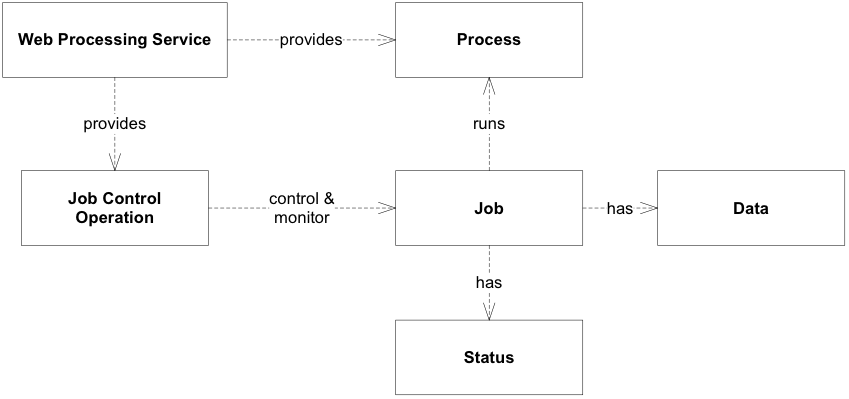
\includegraphics[height=7cm]{pictures/WPS.png}
\caption{Konceptuální model WPS [21]}
\label{fig:wps}
\end{figure}


\section{YAML formát} \label{yaml}



\hspace{10mm}YAML (YAML Ain’t Markup Language) je jazyk pro serializaci dat. Je tvořen tak, aby byl čitelný a pohodlný pro užívání s řadou novodobých programovacích jazyků. Informace uchovává v Unicode charakterů strukturovaných v hodnotových párech a  odrážkových seznamech.  [22]
\begin{figure}[ht] \label{obr7}
\centering

\includegraphics[height=3cm]{pictures/yaml.png}
\caption{Logo projektu YAML  (zdroj: Wikimedia Commons)}
\label{fig:yaml}
\end{figure}

\hspace{10mm}YAML se od XML liší tím, že je vytvořen hlavně pro ukládání dat, zatímco XML slouží k uložený uspořádaných dokumentů. YAML je lépe čitelný díky odsazení a chybějícím znaménkům zatímco XML používá složitější syntaxi. [22]

\hspace{10mm}YAML je také jednoduší pro editaci člověkem než JSON, který je vhodnější pro zpracování strojem. YAML může mít složitější datové struktury a využívá komentáře, ale JSON má jednodušší pravidla. [22]


\section{Python knihovna PyQt} \label{pyqt}
\hspace{10mm}PyQT je sada Python příkazů pro multiplatformní aplikační vývojovou platformu, která kombinuje všechny výhody Qt a Pythonu.  [23]

\begin{figure}[ht] \label{obr8}
\centering

\includegraphics[height=3cm]{pictures/Python_and_Qt.png}
\caption{Kombinace log Python a Qt  (zdroj: Wikimedia Commons)}
\label{fig:qt}
\end{figure}

\hspace{10mm}Qt je aplikační rámec pro tvorbu uživatelských prostředí podporující řadu hardwaru a operačních systémů. Tvorbu uživatelského prostředí podporují softwary jako jsou QtCreator nebo QtDesigner, jehož specializovaná verze je součástí instalace QGIS.

\hspace{10mm}PyQt umožňuje propojit Python kód s množstvím prvků uživatelského prostředí, jako jsou tlačítka, popisky, přepínače, zaškrtávací polička, rozbalovací seznamy nebo okna pro vstup textu.

\section{Python knihovna pytest} \label{pytest}
\hspace{10mm}Robustní knihovna pytest se používá pro všechny druhy testování softwarů. Od konkurenční knihovny unittest na tuto přešla spousta projektů, jakou jsou třeba Mozilla nebo Dropbox. [24]

\begin{figure}[ht] \label{obr9}
\centering

\includegraphics[height=4cm]{pictures/Pytest_logo.png}
\caption{Logo knihovny pytest [24]}
\label{fig:pytest}
\end{figure}

\hspace{10mm}Výhody knihovny jsou například nezávislost na verzi Pythonu, snadná čitelnost a implementace nebo otevřenost zdrojového kódu pod licencí MIT. Díky tomu byla pro knihovnu vyvinuta řada zásuvných modulů pro specifičtější použití.[24]

\hspace{10mm}Testy je možné spouštět přímo v příkazové řádce, přičemž je uživatel informován o prostředí ve kterém je test spuštěn, době jeho trvání a počtu procházejících a selhávajících úkonů.   

\section{GitHub} \label{github}
Tato vývojářská platforma umožňuje vzdálené uložení a editaci kódu. Na její pozadí stojí Git, což je systém pro správu verzí. Ten byl původně vytvořen Linusem Tovaldsem, aby usnadnil vývoj jádra operačního systému Linux. [25]

\begin{figure}[ht] \label{obr10}
\centering

\includegraphics[height=4cm]{pictures/git.png}
\caption{Logo platformy GitHub (vlevo) a systému Git (vpravo) [25]}
\label{fig:git}
\end{figure}

\hspace{10mm}Na stránkách GitHub je možné po založení účtu vytvořit repozitář pro daný projekt. Při vývoji lze vytvářet nové vývojové větve (branch), které je možné zařadit do větve hlavní. Tímto způsobem může na projektu spolupracovat více lidí najednou a nezávisle. Výhodou je také fakt, že v každé větvi je možné provedené změny vrátit do původního stavu. Tento proces lze zjednodušeně přiblížit na úpravě textového dokumentu více uživateli ve službě Google Docs. [25]

\hspace{10mm}Při zapojení (\textit{merge}) vedlejší větve s úpravami do hlavní lze vytvořit žádost o začlenění změn (\textit{pull-request}), kde může více uživatelů diskutovat o provedených změnách. [25]

\hspace{10mm}Github je možné propojit s velkým množstvím vývojových prostředí nebo je možné využít aplikaci GitHub Desktop pro klonování repozitářů na lokální úložiště. Nicméně stejné funkcionality lze dosáhnout užitím pouze
příkazové řádky. [25]

\hspace{10mm}Pomocí služby GitHub Actions lze repozitář propojit s nějakou externí funkcionalitou, mezi které patří: vytvoření Python knihovny, vytvoření Dockeru, propojení s externími cloudovými službami, spouštění testů nebo vytvoření webových stránek ze souborů repozitáře. [25]


\chapter{Postup implementace} \label{implementace}
\hspace{10mm}Všechny kroky implementace byly uskutečněny v rámci GitHub repozitáře v spadající pod organizaci GeoForAll Lab at CTU in Prague.

\section{Návrh pracovního postupu} \label{workflow}
\hspace{10mm}Nejprve bylo nutné zajistit způsob, jakým bude uživatel definovat zájmovou oblast pro průběh analýzy. Vhodně se jevilo, aby bylo možné zvolit oblast buď uvnitř již existujícího polygonu nebo zjednodušeně ve výřezu okna obrazovky.

\hspace{10mm}Geometrické a polohové vlastnosti těchto objektů bylo nutné následně předat službám WPS a WFS zajišťující získávání dat od třetích stran. Po získání vektorových dat ze služeb WFS poskytovaných správci datových sad ZABAGED a LPIS se jevilo žádoucí aplikovat buffer na liniové či bodové prvky s předpokladem že tyto buffery se budou řídit atributovými hodnotami takových vrstev (například třída nebo typ pozemní komunikace). 

\hspace{10mm}Všem polygonovým vrstvám je následně potřeba přiřadit kód využití území. Základní dle názvu vrstvy a detailnější hodnotu dle různých hodnot atributů (příkladem může být třeba vrstva lesa, které byla přidána základní hodnota a přírůstky k této hodnotě dle atributu druhu lesa).

\hspace{10mm}Po těchto úpravách následuje proces oříznutí vrstev, tak aby přesně kopírovaly definiční polygon zájmového území na vstupu a aby prvky po aplikovaném bufferu tento polygon či výřez obrazovky nepřesahovaly.

\hspace{10mm}Dále existuje potřeba tyto vrstvy spojit do jedné dle dané priority. Například tak, aby komunikace vedly nad vodními toky, budovy se nacházely nad zastavěnou plochou a podobně.

\hspace{10mm}Druhou potřebnou vrstvou vstupující do výpočtu je vrstva obsahující hydrologické skupiny půd (HSG). Ta je získávána z WPS služby umístěné na adrese rain.fsv.cvut.cz. Tato služba umožňuje získávat půdní data v rastrové podobě, a proto následuje proces jejich polygonizace. Taková vrstva je také oříznuta dle zájmového území.

\hspace{10mm}Pomocí geometrického sjednocení vstupních prvků jsou obě vrstvy spojeny do jedné se zachovanými atributy o hydrologických skupinách půd a využití území.
Z jejich kombinace se poté dle zvolené tabulky přiřadí hodnoty CN.

...

\begin{figure}[H] \label{obr11}
\centering
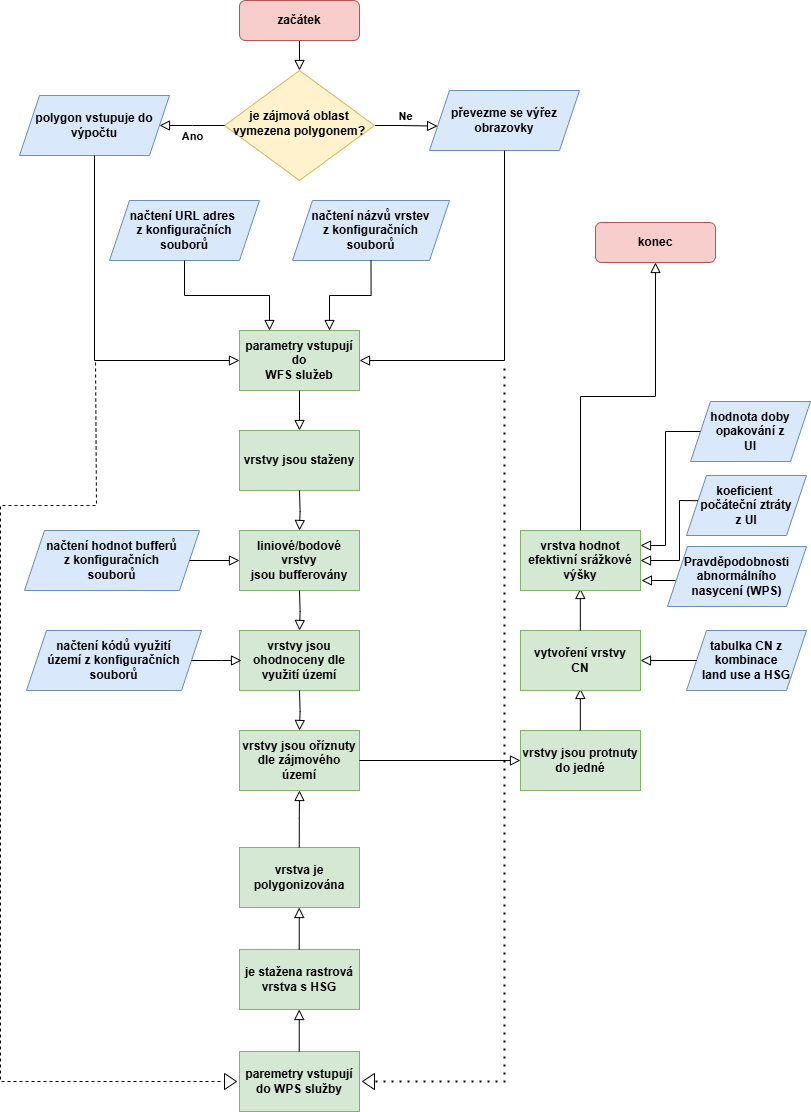
\includegraphics[height=21cm]{pictures/diagram.png}
\caption{Vývojový diagram pracovního postupu}
\label{fig:diagram}
\end{figure}

\section{Tvorba grafického uživatelského rozhraní} \label{gui}
\begin{figure}[H] \label{obr12}
\centering

\includegraphics[height=2cm]{pictures/icon.png}
\caption{Ikona zásuvného modulu}
\label{fig:icon}
\end{figure}

\section{Získávání vrstvy využití území (land use)} \label{landuse}
\hspace{10mm}Nejprve je nutné získat územní rozsah ve kterém se budou získávat potřebné vrstvy. Podle volby uživatele v grafickém uživatelském rozhraní se použije buď výřez obrazovky nebo ohraničující obdélník vybraného polygonu.  
\begin{lstlisting}[style=mypython, caption={Získání územního rozsahu}, label={kod:extent}]
if not self.AreaFlag:
    extent = iface.mapCanvas().extent()
elif self.polygon and self.polygon.isValid():
    extent = self.polygon.extent()
else:
    QgsMessageLog.logMessage("Invalid polygon layer!", 
    "CzLandUseCN", level=Qgis.Warning, notifyUser=True)
\end{lstlisting}

\hspace{10mm}Z konfiguračních souborů je poté načten seznam názvů a URL adresy WFS služeb stahovaných vrstev. Všechny tyto parametry jsou přesunuty do jiného vlákna QGISU, kvůli zachování responsivity samotné aplikace QGIS při procesu stahování. Na pozadí je potom stažena z WFS služby každá vrstva z dříve získaného seznamu vrstev v požadovaném rozsahu. Každou získanou vrstvou se také přiřadí nová hodnota v ukazateli průběhu v uživatelském rozhraní.

\begin{lstlisting}[style=mypython, caption={Stažení vrstvy z WFS služby}, label={kod:wfs}]
def process_wfs_layer(self, layer_name: str, ymin: float, xmin: float, ymax: float, xmax: float,
  extent: QgsGeometry,
  URL: str) -> Optional[QgsVectorLayer]:
""" Load and clip a WFS layer to the given extent"""
uri = (
f"{URL}?"
f"&version=2.0.0&request=GetFeature&typename={layer_name}"
f"&bbox={xmin},{ymin},{xmax},{ymax},EPSG:5514"
)

vlayer = QgsVectorLayer(uri, f"Layer: {layer_name}", "WFS")

clipped_layer = self.clip_layer(vlayer, extent, layer_name)
if clipped_layer.isValid():
	return clipped_layer
\end{lstlisting}
\hspace{10mm}Takto získané vrstvy se uchovají v paměti počítače a nyní je potřeba provést kroky, aby jednotlivé vrstvy reprezentovaly využití území. K jednoznačné identifikaci typu využití území se využije kód, který se zároveň bude vyskytovat v tabulce pozdější funkcionality určení hodnoty CN. V první fázi přiřazení se u každé vrstvy vytvoří atribut pro hodnotu kódu využití území a doplní se jeho základní hodnota dle názvu vrstvy. Rozlišné vrstvy mohou mít i totožný kód využití území, jako například silnice a parkoviště, jelikož se v obou případech jedná o antropogenní nepropustné povrchy. Tato hodnota je přiřazena pomocí klíčového slova v názvu vrstvy, ke kterému je v konfiguračním souboru přiřazena hodnota kódu využití území. Díky tomu bude tato funkcionalita zachována i v případě, že správce WFS služby obmění názvy poskytovaných vrstev.

\begin{lstlisting}[style=mypython, caption={Přiřazení kódu využití území}, label={kod:landusecode}]
for entry in data["land_use"]:
    names = entry["keywords"]  # Get keyword list
    code = entry["code"]  # Get land use code

    if any(name.lower() in layer_name.lower() for name in names):
        layer.startEditing()
        for feature in layer.getFeatures():
            feature["LandUse_code"] = code
            layer.updateFeature(feature)
        layer.commitChanges()

updated_layers.append(layer)  # Always append the layer
return updated_layers
\end{lstlisting}

\hspace{10mm}Některé stahované vrstvy jsou liniové nebo bodové a právě na ty je aplikován buffer. Pro mnohé je aplikován jen pouze dle názvu vrstvy a pro některé je hodnota bufferu přiřazena dle vybraného řídícího atributu. Pokud řídící atribut obsahuje nečekané hodnoty nebo neobsahuje hodnotu žádnou, je zvolena definovaná implicitní velikost bufferu.

\begin{lstlisting}[style=mypython, caption={Přiřazení velikosti bufferu}, label={kod:buffer}]
for feature in layer.getFeatures():
    value = feature[controlling_atr_name]
    if value in flat_values:
        index = flat_values.index(value)
        buffer_distance = distances[index // len(values[0])]
    else:
        buffer_distance = default_buffer
\end{lstlisting}

\hspace{10mm}Další implementovanou funkcí pluginu je zpřesnit kód využití území dle nějakého atributu vrstvy. Jelikož atribut u vrstvy nemění přiřazený kód z názvu vrstvy, tak se k již přiřazené hodnotě pouze přičte žádané číslo. Jestliže atribut obsahuje neočekávanou hodnotu, zůstane u prvku pouze základní kód.

 \hspace{10mm}Po těchto úpravách je na řadě oříznutí vrstev tak, aby po aplikovaném bufferu nezasahovaly mimo zájmové území. Následně je potřeba všechny vrstvy spojit do jedné podle požadovaného pořadí. Na finální spojenou vrstvu využití území je pak aplikována tabulka symbologie a je přidána do projektu.
 
\section{Získání vrstvy HSP a její propojení s vrstvou využití území} \label{intersection}
 \hspace{10mm}Data hydrologických skupin půd využitých v zásuvném modulu jsou získávány z WPS služby umístěné na doméně \textit{rain.fsv.cvut.cz} . Tato služba má na vstupu polygonovou vrstvu s maximálním rozsahem 20 km a názvy požadovaných vrstev. Tato služba totiž nabízí kromě dat hydrologických skupin půd i míru zastoupení písku, naplavenin, jílu a texturu půdy podle USDA. Nicméně tyto další poskytované vrstvy nejsou ve výpočtu využity. Všechny tyto vrstvy poskytovány v rastrové podobě byly vytvořeny v rámci projektu Fyzikální a hydropedologické vlastnosti půd ČR.

 \hspace{10mm}Zájmová oblast je uživatelem zadávána stejně jako u dat získávaných pro vrstvu využití území buď polygonem nebo výřezem obrazovky, a proto musí být v druhém případě tento vstup převeden do polygonu.  
\begin{lstlisting}[style=mypython, caption={Převod výřezu obrazovky na polygon},label={kod:extenttoplg}]
rect = QgsRectangle(xmin, ymin, xmax, ymax)
layer = QgsVectorLayer("Polygon?crs=EPSG:5514", "Rectangle Layer", "memory")
provider = layer.dataProvider()
fields = QgsFields() # Define attributes
fields.append(QgsField("id", QVariant.Int))
provider.addAttributes(fields)
layer.updateFields()
feature = QgsFeature() # Create a feature with rectangle geometry
feature.setGeometry(QgsGeometry.fromRect(rect))
feature.setAttributes([1])  # Assign an ID
provider.addFeature(feature)
layer.updateExtents()# Refresh the layer
return layer
\end{lstlisting}

 \hspace{10mm}Tato služba WPS vrací pouze matici pixelů, které jsou v celém rozsahu uvnitř definičního polygonu, proto aby byly použity pixely na obvodu polygonu je na vstupní polygon aplikován buffer o hodnotě dvojnásobném rozlišení rastrové vrstvy. 

 \hspace{10mm} Jelikož po předání vektorové vrstvy WPS službě tato služba stahuje data uvnitř geometrií každého prvků této vrstvy je pro urychlení procesu na vrstvu aplikována funkce sloučení \textit{(dissolve)}, tak aby byly předány pouze souřadnice vrcholových bodů celé vrstvy, což také zjednodušuje kontrolu celkového rozsahu zájmového území.

  \hspace{10mm} Pro komunikaci se službou je potřeba jí předat požadavek ve formátu XML. To se vytvoří doplněním ohraničujícího obdélníku, body a atributy definičního polygonu do XML šablony uložené ve složce s konfiguračními soubory. Toto XML se předá s identifikátorem pro stažení vrstvy hydrologických skupin půd funkci \textit{(execute)} knihovny OWSLib.
\begin{lstlisting}[style=mypython, caption={Spuštění kominukace s WPS službou},label={kod:wps}]
execution = wps.execute(self.process_identifier, [], request=requestXML.encode('utf-8'))
monitorExecution(execution)
\end{lstlisting}

\hspace{10mm}Výstupem služby je rastrová vrstva v komprimované složce, ta je uložena do dočasné složky vytvořené v systému. Ta je poté extrahována a soubor formátu TIF je uložen do paměti počítače. Ten je polygonizací převeden do vektorové podoby a uložen do stejné dočasné složky ve formátu GeoPackage.

\begin{lstlisting}[style=mypython, caption={Polygonizace rastrové vrstvy},label={kod:polygonizace}]
temp_output = tempfile.NamedTemporaryFile(suffix=".gpkg").name
result = processing.run("gdal:polygonize", {
    'INPUT': raster_path,
    'BAND': 1,
    'FIELD': 'HSG',
    'EIGHT_CONNECTEDNESS': False,
    'OUTPUT': temp_output })
\end{lstlisting}

\hspace{10mm}Vektorová vrstva je poté oříznuta dle původního polygonu na vstupu, na který nebyl aplikován buffer. Nicméně tato vrstva HSP může obsahovat díry. To nastává hlavně na místech, kde se nachází nějaká vodní plocha. Takové díry jsou poté vyplněny hodnotou 0 a je s nimi nakládáno jako s vodní plochou. Na výslednou vrstvu je aplikován barevný styl.

\hspace{10mm}Po přidání vrstvy využití území i vrstvy hydrologických skupin se tyto vrstvy zároveň propojí s rozevíracími seznamy na druhé záložce v grafickém uživatelském rozhraní. Odtud je potom možné obě vrstvy propojit do jedné.

\hspace{10mm}Pokud je jedna z vrstev rozsahem větší než druhá, je ta větší oříznuta dle té menší. Vrstvy jsou potom i s atributy spojeny do jedné a je na ně aplikována symbologie.

\begin{lstlisting}[style=mypython, caption={Propojení vrstev využití území a HSP},label={kod:intersection}]
combined_layer = processing.run("native:union", {
                'INPUT': self.LandUse_layer,
                'OVERLAY': self.Soil_layer,
                'OUTPUT': 'memory:'
            })['OUTPUT']
\end{lstlisting}



\section{Analýza odtoků SCS-CN} \label{CN}
\section{Výpočet objemu přímého odtoku} \label{runoff}
\section{Popis konfiguračních souborů} \label{config}
\subsection{layers\_merging\_order.csv} \label{layers_merging_order.csv}
\hspace{10mm}Tento jednoduchý csv soubor obsahuje v každém řádku název vrstvy poskytované ZABAGED WFS službou. Jejich pořadí určuje pořadí, ve kterém budou spojeny do jedné vrstvy využití území. Vrstvy uvedené dříve budou připojeny nad vrstvy pod nimi. označení \textit{LPIS\_layer} neslouží ke stažení vrstvy, ale pouze určuje pořadí vrstvy z WFS LPIS služby.

\begin{lstlisting}[style=mypython, caption={Ukázka layers\_merging\_order.csv},label={kod:layers_merging_order.csv}]
ZABAGED_POLOHOPIS:Heliport
ZABAGED_POLOHOPIS:Budova_jednotlivá_nebo_blok_budov__plocha_
ZABAGED_POLOHOPIS:Silnice__dálnice
LPIS_layer
ZABAGED_POLOHOPIS:Okrasná_zahrada__park
\end{lstlisting}


\subsection{zabaged\_to\_LandUseCode\_table.yaml} \label{zabaged_to_LandUseCode_table.yaml}
\hspace{10mm}Toto je YAML soubor, který obsahuje seznam obsahující mapy vždy s dvěma stejnými klíči \textit{keywords} a \textit{code}. \textit{Keywords} obsahuje seznam řetězců a \textit{code} jedno celé číslo.

\hspace{10mm}Soubor je využit k mapování kódů využití území. Pokud se alespoň jedne řetězec uvnitř seznamu \textit{keywords} nachází v názvu získané ZABAGED vrstvy, je takové vrstvě přiřazen kód využití území z korespondujícího klíče \textit{code}.

\hspace{10mm}Tento postup je volen tak, aby při změně názvů vrstev poskytovatelem bylo toto přiřazení stále funkční.

\begin{lstlisting}[style=myyaml, caption={Ukázka zabaged\_to\_LandUseCode\_table.yaml},label={kod:zabaged_to_LandUseCode_table.yaml}]
land_use:
  - keywords: [Orná, orná, Orna, orna]
    code: 10000
  - keywords: [Travní, travní, Travni, travni]
    code: 20000
  - keywords: [Lesní, lesní, Lesni, lesni]
    code: 30000
\end{lstlisting}

\subsection{ZABAGED.yaml} \label{ZABAGED.yaml}
\hspace{10mm} Tento soubor obsahuje informace o vrstvách stahovaných ze ZABAGED WFS služby a slouží k jejich úpravě. Jmenovitě to je aplikace bufferu a zpřesnění kódu využití území.

\hspace{10mm}Na prvním řádku soubor obsahuje URL adresu v řetězci pod klíčem \textit{URL}, kde se nachází WFS služba poskytující ZABAGED data.Dále seznam vrstev, pro které se mají vytvářet buffery podle určitých hodnot v atributech. Každý objekt obsahuje sadu klíčů.

\hspace{10mm}První \textit{input\_layer\_name} obsahuje název stažené WFS vrstvy, \newline \textit{controlling\_atr\_name} název atributu dané vrstvy podle kterého se řídí přiřazení bufferu, \textit{default\_buffer} který se přiřazuje pokud žádný atribut vrstvy neodpovídá žádnému v tomto souboru a \textit{buffer\_levels} obsahující tři úrovně \textit{priority}, \textit{values} a \textit{distance}.

\hspace{10mm}Klíč \textit{priority} obsahuje číselný řetězec pro určení pořadí při výběru hodnot, klíč \textit{values} hodnoty v atributu, které spadají do této úrovně a \textit{distance} obsahuje vzdálenost bufferu v metrech.

\hspace{10mm}Pokud \textit{controlling\_atr\_name} není poskytnut, potom se všem objektům vrstvy přiřadí velikost buffer z hodnoty \textit{default\_buffer}.

\hspace{10mm}Další seznam obsahuje názvy vrstev, pro které je žádoucí zpřesnit hodnotu kódu pod klíčem \textit{name}. Dále pak základní hodnotu kódu využití území \textit{base\_use\_code}. Ten je zde znovu přiřazen pro případ, že není přiřazen ze souboru  \newline \textit{zabaged\_to\_LandUseCode\_table.yaml}. Opět se tu nachází název \textit{controlling\_attribute}, který musí vrstva na vstupu obsahovat a dle jeho hodnot se přičte celočíselná hodnota ze seznamu \textit{value\_increments}, kde se nachází pod klíčem totožným s hodnotou atributu vrstvy. 

\begin{lstlisting}[style=myyaml, caption={Ukázka ZABAGED.yaml},label={kod:ZABAGED.yaml}]
URL: "https://ags.cuzk.cz/arcgis/services/ZABAGED_POLOHOPIS/MapServer/WFSServer"

buffer_layers:
  - input_layer_name: "ZABAGED_POLOHOPIS:Silnice__dálnice"
    controlling_atr_name: "typsil_k"
    buffer_levels:
      - priority: "1"
        values: ["D1", "D2", "M", "D1p", "Mp", "Mv"]
        distance: 20
      - priority: "2"
        values: ["S1", "S1v", "S1p"]
        distance: 12.5
      - priority: "3"
        values: ["S2", "S3", "D2p", "S2p", "S2v", "S3p", "S3v"]
        distance: 10
    default_buffer: 7.5

  - input_layer_name: "ZABAGED_POLOHOPIS:Silnice_neevidovaná"
    controlling_atr_name: "NaN"
    default_buffer: 7.5

layers:
  - name: "ZABAGED_POLOHOPIS:Lesní_půda_se_stromy_kategorizovaná__plocha_"
    base_use_code: 30000
    controlling_attribute: "druh_k"
    value_increments:
      N: 0
      J: 3200 # jehlicnaty
      L: 3100 # listnaty
      S: 3300 # smiseny
\end{lstlisting}

\subsection{LPIS.yaml} \label{LPIS.yaml}
\hspace{10mm} \textit{LPIS.yaml} obsahuje informace o vrstvě stahované z LPIS WFS služby. Pod klíčem \textit{URL} se obdobně jako u souboru \textit{ZABAGED.yaml} nachází adresa k LPIS WFS. Z té je stahována pouze jedna vrstva a její název je uložen pod klíčem \textit{layer\_name}.

\hspace{10mm} Aby bylo možné použít totožný proces editace kódu využití území jako u ZABAGED vrstev, je dále v listu \textit{layers}  uložen název vrstvy v klíči \textit{name}. Ten je definován jako \textit{LPIS\_layer}, který je stahované vrstvě dříve přiřazen, aby byla spojena s ostatními vrstvami ve správném pořadí dle souboru popsaném v části 5.7.2.

\hspace{10mm}Ze stejného důvodu je také přiřazena základní hodnota kódu využití území pod klíčem \textit{base\_use\_code}, název řídícího atributu \textit{controlling\_attribute}, který je očekáván ve stahované vrstvě a dále seznam \textit{value\_increments} s hodnotovými páry, kde klíčem je hodnota atributu vrstvy. Dle klíče je přiřazen přírůstek k základní hodnotě \textit{base\_use\_code}.

\begin{lstlisting}[style=myyaml, caption={Ukázka LPIS.yaml},label={kod:LPIS.yaml}]
URL: "https://mze.gov.cz/public/app/wms/plpis_wfs.fcgi"
layer_name: "LPIS_DPB_UCINNE"

layers:
  - name: "LPIS_layer"
    base_use_code: 10000
    controlling_attribute: "kultura"
    value_increments:
      "standartní orná půda": 0
      "chmelnice": 3100
      "vinice": 3200
\end{lstlisting}

\subsection{Soil.yaml} \label{Soil.yaml}
Tento soubor obsahuje pouze dvě hodnotové páry, a to \textit{URL} s adresou WPS služby poskytující data HSP a \textit{process\_identifier} který obsahuje řetězec , který obsahuje název požadované vrstvy stahované z této služby.


\subsection{Soil\_template.xml} \label{Soil_template.xml}
\hspace{10mm} Tento soubor obsahuje šablonu XML souboru pro komunikaci s WPS službou stahující vrstvu hydrologických skupin půd.
Do této šablony jsou před odesláním WPS službě doplněny hodnoty souřadnic definičního polygonu, souřadnice jeho ohrazujícího obdélníku a jeho atributy.


\section{Kontroly} \label{checks}
\section{Testování} \label{testing}
\section{Tvorba dokumentace} \label{docs}

\clearpage  % SEM NESAHEJTE!
\addcontentsline{toc}{chapter}{Seznam použité literatury}  \label{zdroje}

\begin{thebibliography}{1}
\bibitem{MNYDGwleJOjKLRUp}
PONCE, V. M. and HAWKINS R. H. 1996. Runoff curve number: Has it reached maturity?
\textit{ Journal of Hydrologic Engineering 1(1):11-19. Dostupné z: \href{https://ponce.sdsu.edu/runoff11view.html}
{https://ponce.sdsu.edu/runoff11view.html}}

\bibitem{Holman2003}
HOLMAN, I.P.; HOLLIS, J.M.; BAMLEY, M.E. a THOMPSON, T.R.E. The contribution of soil structural degradation to catchment flooding: a preliminary investigation of the 2000 floods in England and Wales. \textit{Hydrology and earth system sciences}. 2003, roč. 7, č. 5, s.~754-765.

\bibitem{Lian2020}
LIAN, Huishu; YEN, Haw; HUANG, Jr-Chuan; FENG, Qingyu; QIN, Lihuan et al. CN-China: Revised runoff curve number by using rainfall-runoff events data in China. \textit{Water Research}. 2020, roč. 2020, č. 177, s.~115767. ISSN 0043-1354. Dostupné také z: \url{https://www.sciencedirect.com/science/article/pii/S0043135420303043}.

\bibitem{MNYDGwleJOjKdRUp}
JANEČEK, Miloslav. Ochrana zemědělské půdy před erozí: metodika.
\textit{ Praha: Powerprint, 2012. ISBN 978-80-87415-42-9. }

\bibitem{MNYDGwleJOjKLRU2}
KAVKA, Petr a KAŠPAR, Marek. Krátkodobé srážky pro hydrologické modelování a navrhování drobných vodohospodářských staveb v krajině: Certifikovaná metodika.
\textit{ Fakulta stavební ČVUT v Praze, 2023. ISBN 978-80-01-07115-1}

\bibitem{MNYDGwleJOjKLRU3}
JANEČEK, M. a P. KOVÁŘ. Aktuálnost „Metody čísel odtokových křivek –
CN“ k určování přímého odtoku z malého povodí.
\textit{ Vodní hospodářství. 2010,
č. 7, s. 187-189.} 

\bibitem{MNYDGwleJOjKLRU5}
Urban hydrology for small watersheds: Technical Release 55 (TR-55) (Second ed.).
\textit{ Natural Resources Conservation Service. Conservation Engineering Division, 1986.}


\bibitem{dONaeOjXanl1W2md}
ČSN P ISO/TS 19104, \textit{Geografická informace - Terminologie}. 2010.

\bibitem{Matejova2019}
MATEJOVÁ, Vlasta. \textit{Quantum GIS}. Diplomová práce. České Budějovice: Jihočeská univerzita v Českých Budějovicích, Ekonomická fakulta, 2019.

\bibitem{Baghdadi2018}
BAGHDADI, Nicolas; MALLET, Clément a ZRIBI, Mehrez. \textit{QGIS and Generic Tools}. Volume 1. John Wiley \& Sons, 2018. ISBN 9781119457091.

\bibitem{QPwvEntkWdxPk0Lz}
QGIS DEVELOPMENT TEAM. \textit{QGIS geographic information system}. Online. 2025. Dostupné z: \url{https://www.qgis.org}. [cit. 2025-01-26].

\bibitem{nEFEg7XpI9hVQCiO}
\textit{Katalog objektů ZABAGED®}. Verze 4.4. Zeměměřický úřad, 2024.


\bibitem{Devaty2018}
DEVÁTÝ, Jan. \textit{Klasifikace území pro erozní modely pomocí GIS a veřejně dostupných datových zdrojů}. Disertační práce. Praha: České vysoké učení technické v Praze, Fakulta stavební, Katedra hydromeliorací a krajinného inženýrství, 2018.

\bibitem{KocurBera2019}
KOCUR-BERA, Katarzyna. Data compatibility between the Land and Building Cadaster (LBC) and the Land Parcel Identification System (LPIS) in the context of area-based payments: A case study in the Polish Region of Warmia and Mazury. \textit{Land Use Policy}. 2019, roč. 2019, č. 80, s.~370-379. ISSN 0264-8377.

\bibitem{sSYEwLE0rNKoWGYk}
\textit{Nařízení vlády č. 307/2014 Sb. o stanovení podrobností evidence využití půdy podle uživatelských vztahů}. 2014. Dostupné také z: \url{http://www.zakonyprolidi.cz/cs/2014-307}.

\bibitem{Strouhal2022}
STROUHAL, Luděk a KAVKA, Petr. Hydrologické skupiny půd --- rozevřené nůžky hydrologických výpočtů (2. část). \textit{Vodní hospodářství}. 2022, roč. 72, č. 9, s.~7-12.

\bibitem{Vretanos2014}
VRETANOS, Panagiotis (Peter) A. \textit{OpenGIS Web Feature Service 2.0 Interface Standard --- With Corrigendum}. 2.0.2. Open Geospatial Consortium, 2014.

\bibitem{Zhang2005}
ZHANG, Chuanrong a LI, Weidong. The Roles of Web Feature and Web Map Services in Real-time Geospatial Data Sharing for Time-critical Applications. Online. \textit{Cartography and Geographic Information Science}. 2005, roč. 32, č. 4, s.~269-283. ISSN 1523-0406. Dostupné z: \url{https://doi.org/10.1559/152304005775194728}. [cit. 2025-02-25].

\bibitem{Schall2009}  
SCHALL, Gerhard, MENDEZ, Erick, KRUIJFF, Ernst, VEAS, Eduardo, JUNGHANNS, Sebastian, REITINGER, Bernhard a SCHMALSTIEG, Dieter.  
Handheld Augmented Reality for underground infrastructure visualization.  
\textit{Personal and Ubiquitous Computing}, 2009, roč. 13, s. 281-291.  
DOI: 10.1007/s00779-008-0204-5.  

\bibitem{Stollberg2007}
STOLLBERG, Beate a ZIPF, Alexander. OGC Web Processing Service Interface for Web Service Orchestration Aggregating Geo-processing Services in a Bomb Threat Scenario. In: J. WARE, Mark, E. TAYLOR, George (ed.). \textit{Web and Wireless Geographical Information Systems}. Anglie, Cardiff: Springer, 2007, s.~239-251. ISBN 978-3-540-76923-1.

\bibitem{5Xjhvf3W3tsG6nhX}
\textit{OGC® WPS 2.0.2 Interface Standard Corrigendum 2}. 2.0.2. Open Geospatial Consortium, 2015.

\bibitem{hsOq0virmVAO85Ud}
BEN-KIKI, Oren; EVANS, Clark a DÖT NET, Ingy. \textit{YAML Ain-t Markup Language (YAML) Version 1.2}. 3rd Edition, Patched at 2009-10-01.

\bibitem{Summerfield2007}
SUMMERFIELD, Mark. \textit{Rapid GUI Programming with Python and Qt: The Definitive Guide to PyQt Programming}. Pearson Education, 2007. ISBN 978-0132703062.

\bibitem{Okken2017}
OKKEN, Brian. \textit{Python Testing with pytest: Simple, Rapid, Effective, and Scalable}. Pragmatic Bookshelf, 2017. ISBN 9781680502404.

\bibitem{Guthals2023}
GUTHALS, Sarah. \textit{GitHub\texorpdfstring{\textsuperscript{\textregistered}}{ (R)} For Dummies \texorpdfstring{\textsuperscript{\textregistered}}{(R)}}. 2nd Edition. Hoboken, New Jersey: John Wiley \& Sons, 2023. ISBN 978-1-394-15917-8.

\end{thebibliography}
\end{document}

